%!TEX encoding = UTF-8 Unicode

\section{Introduction}

% TODO: delete the seq2-* png files (view from external camera)
% \begin{figure*}
%     \centering
%     \subfloat
%     { 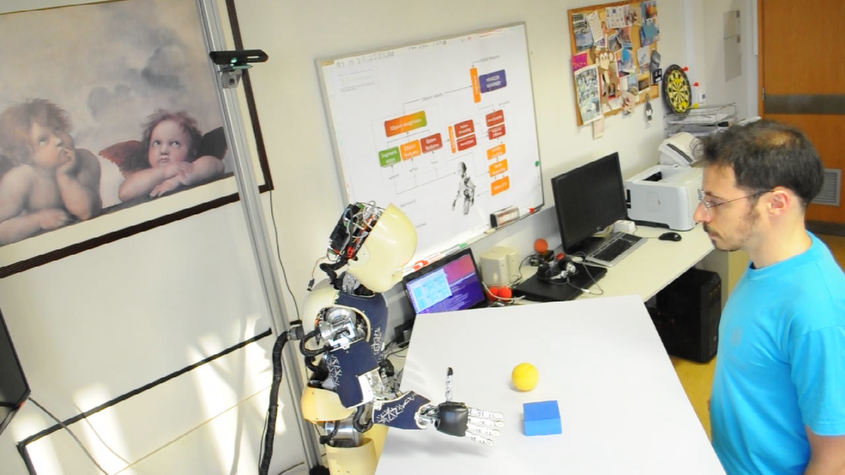
\includegraphics[width=\myWidth\linewidth]{seq2-grasp-11} } \quad
%     %
%     \subfloat
%     { 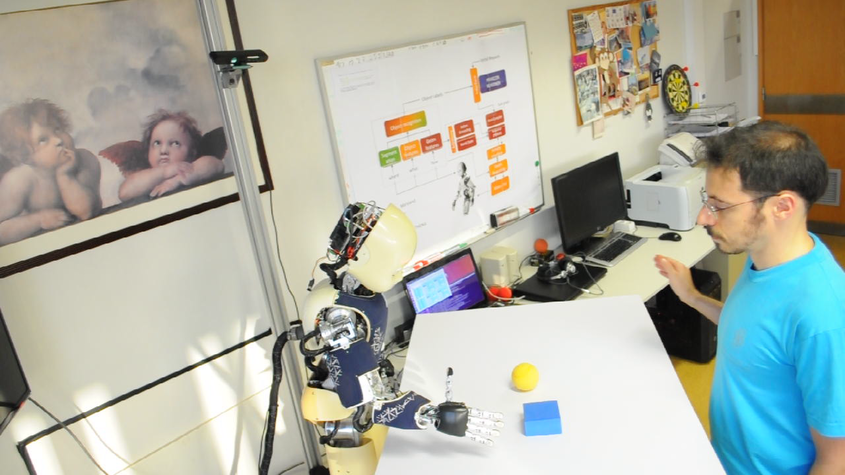
\includegraphics[width=\myWidth\linewidth]{seq2-grasp-12} } \quad
%     %
%     \subfloat
%     { 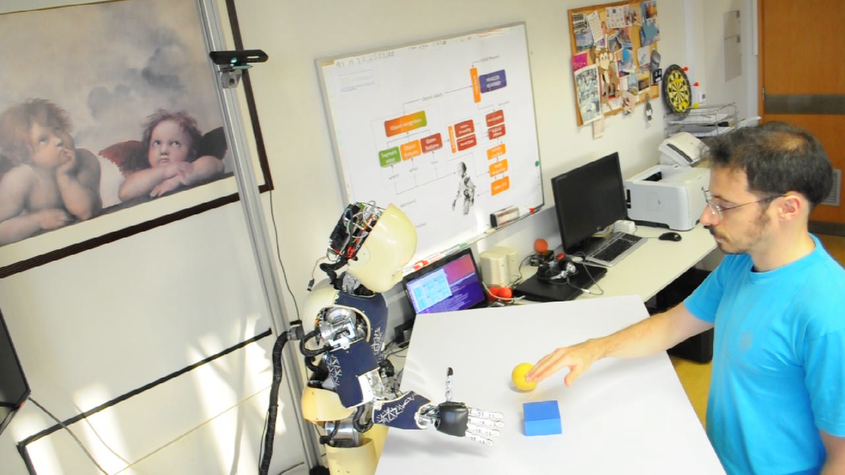
\includegraphics[width=\myWidth\linewidth]{seq2-grasp-13} } \\
%     %
%     \subfloat
%     { 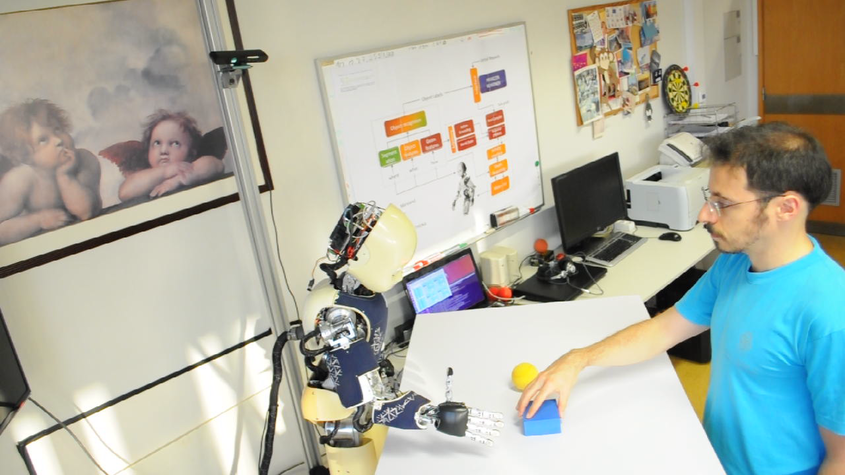
\includegraphics[width=\myWidth\linewidth]{seq2-grasp-14} } \quad
%     %
%     \subfloat
%     { 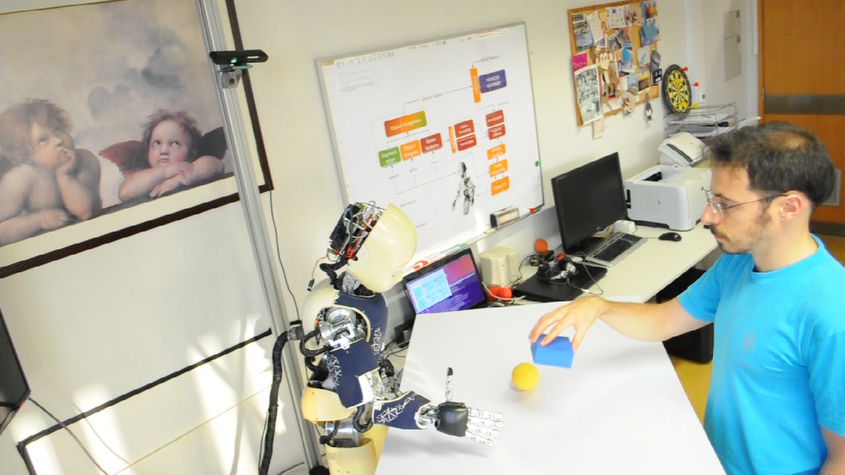
\includegraphics[width=\myWidth\linewidth]{seq2-grasp-15} } \quad
%     %
%     \subfloat
%     { 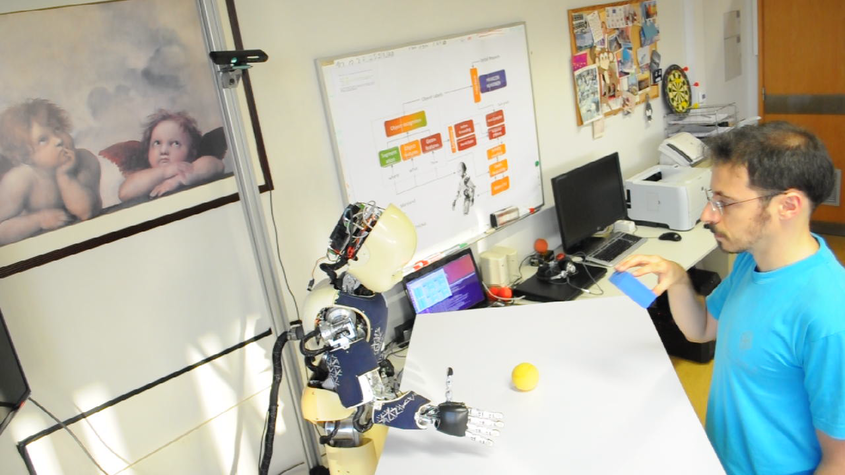
\includegraphics[width=\myWidth\linewidth]{seq2-grasp-16} }
%     \caption{grasp}
% \end{figure*}
%
% \begin{figure*}
%     \centering
%     \subfloat
%     { 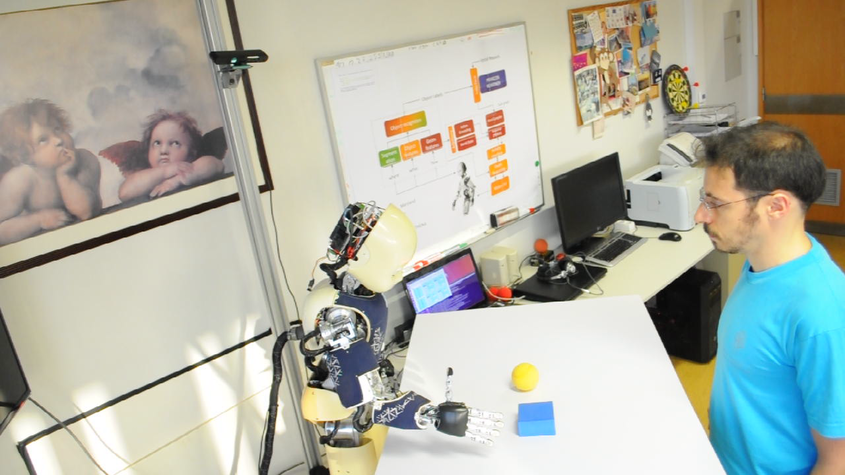
\includegraphics[width=\myWidth\linewidth]{seq2-tap-22} } \quad
%     %
%     \subfloat
%     { 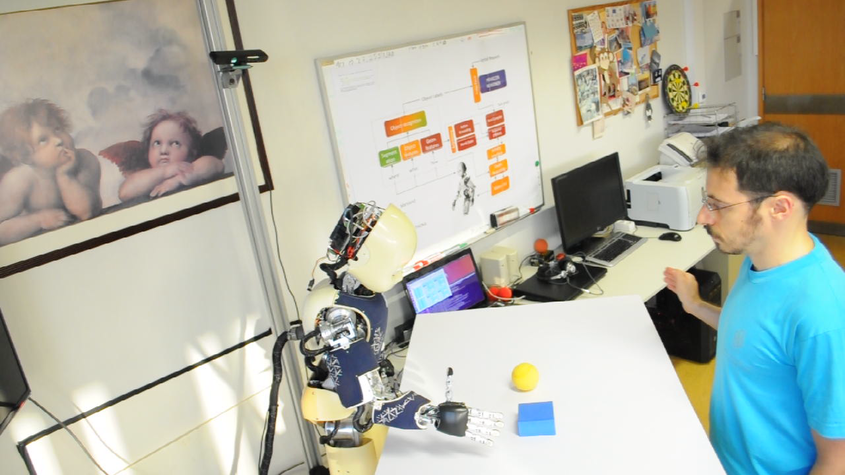
\includegraphics[width=\myWidth\linewidth]{seq2-tap-23} } \quad
%     %
%     \subfloat
%     { 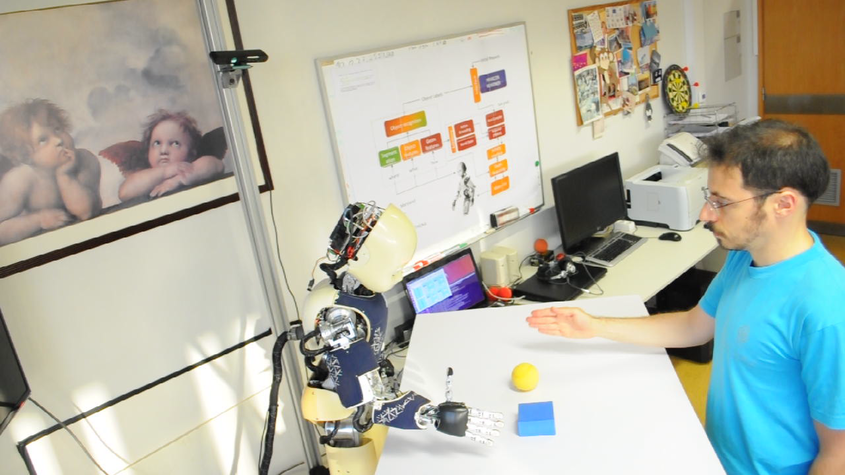
\includegraphics[width=\myWidth\linewidth]{seq2-tap-24} } \\
%     %
%     \subfloat
%     { 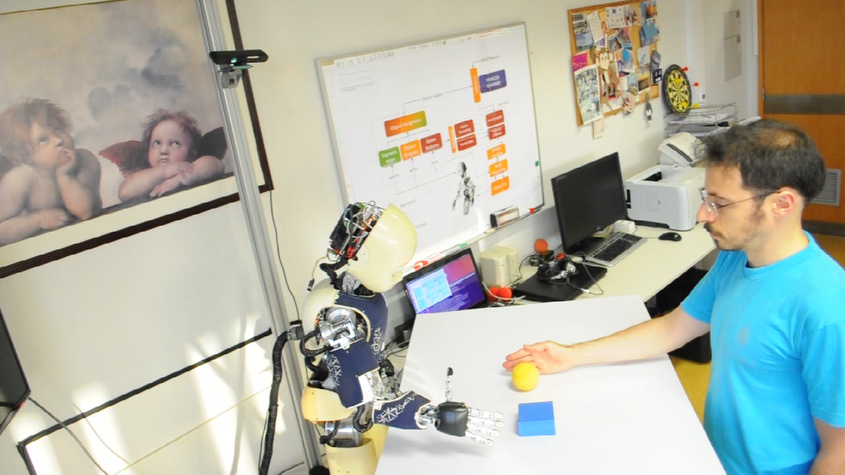
\includegraphics[width=\myWidth\linewidth]{seq2-tap-25} } \quad
%     %
%     \subfloat
%     { 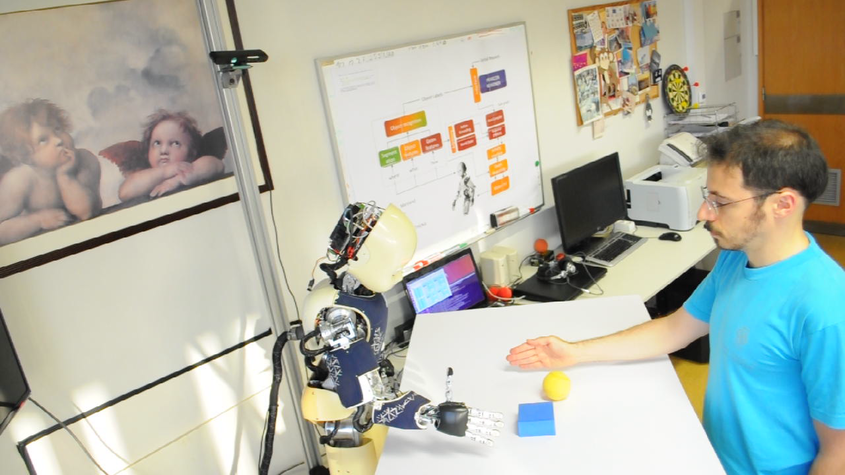
\includegraphics[width=\myWidth\linewidth]{seq2-tap-26} } \quad
%     %
%     \subfloat
%     { 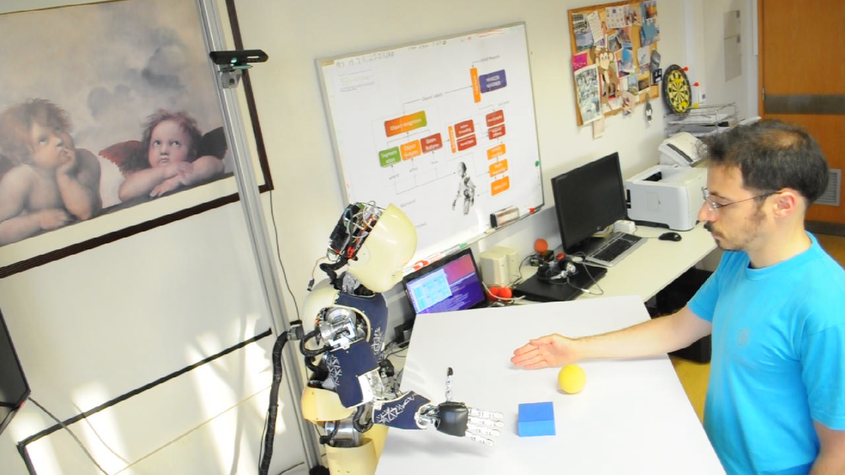
\includegraphics[width=\myWidth\linewidth]{seq2-tap-27} }
%     \caption{tap}
% \end{figure*}
%
% \begin{figure*}
%     \centering
%     \subfloat
%     { 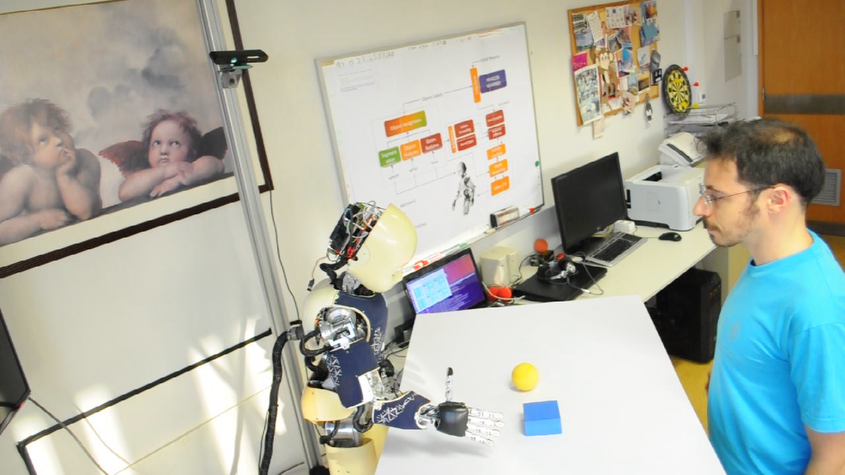
\includegraphics[width=\myWidthTwo\linewidth]{seq2-touch-2} } \quad
%     %
%     \subfloat
%     { 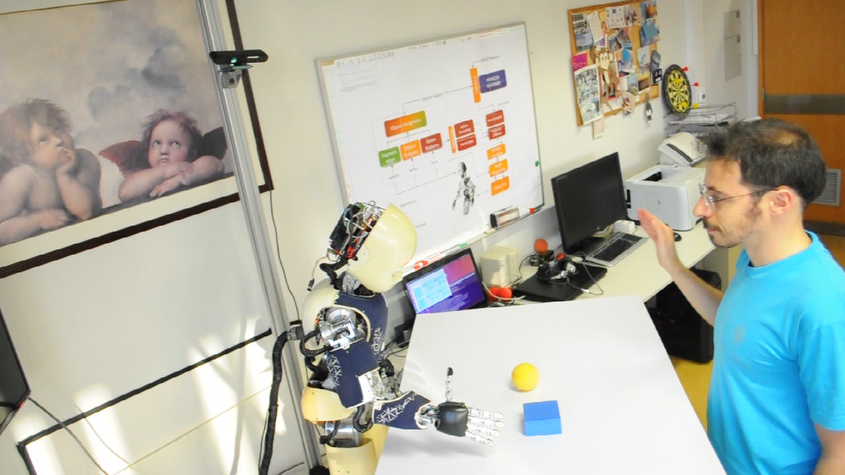
\includegraphics[width=\myWidthTwo\linewidth]{seq2-touch-3} } \quad
%     %
%     \subfloat
%     { 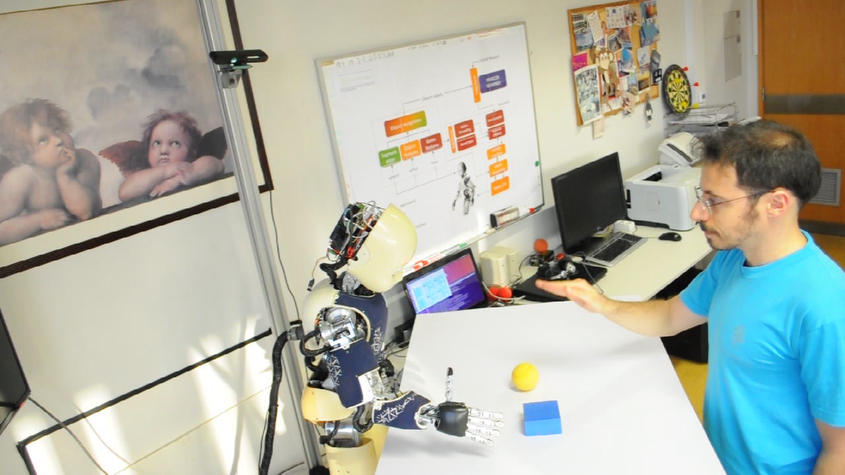
\includegraphics[width=\myWidthTwo\linewidth]{seq2-touch-4} } \quad
%     %
%     \subfloat
%     { 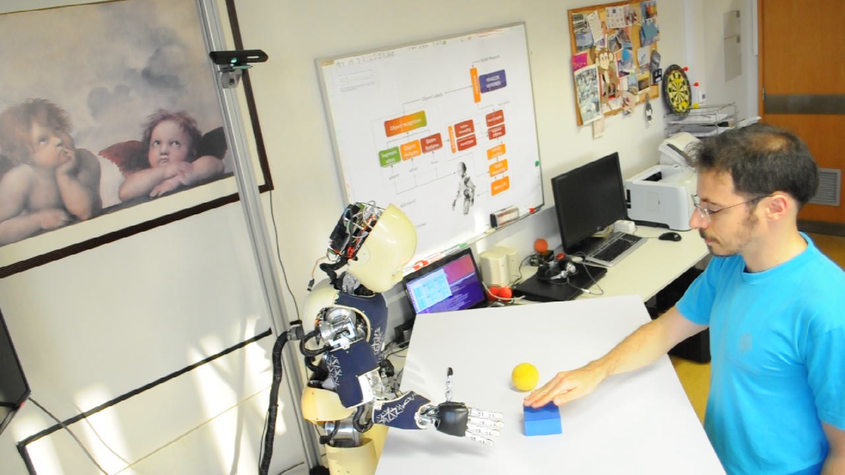
\includegraphics[width=\myWidthTwo\linewidth]{seq2-touch-5} } \\
%     %
%     \subfloat
%     { 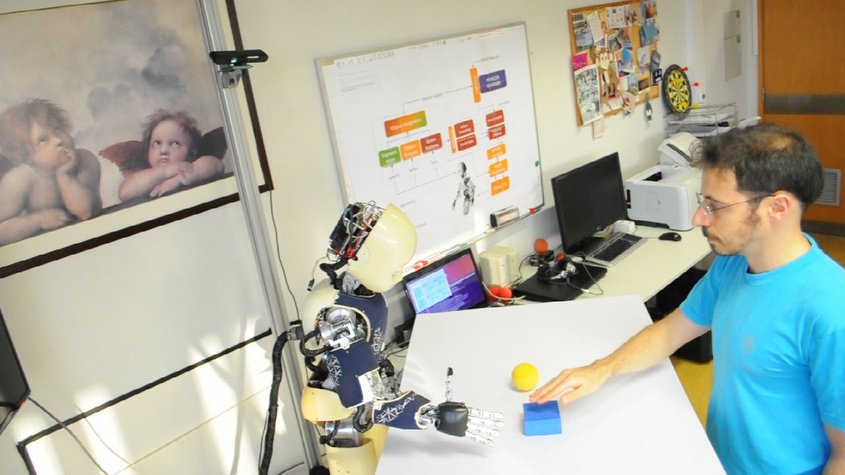
\includegraphics[width=\myWidthTwo\linewidth]{seq2-touch-6} } \quad
%     %
%     \subfloat
%     { 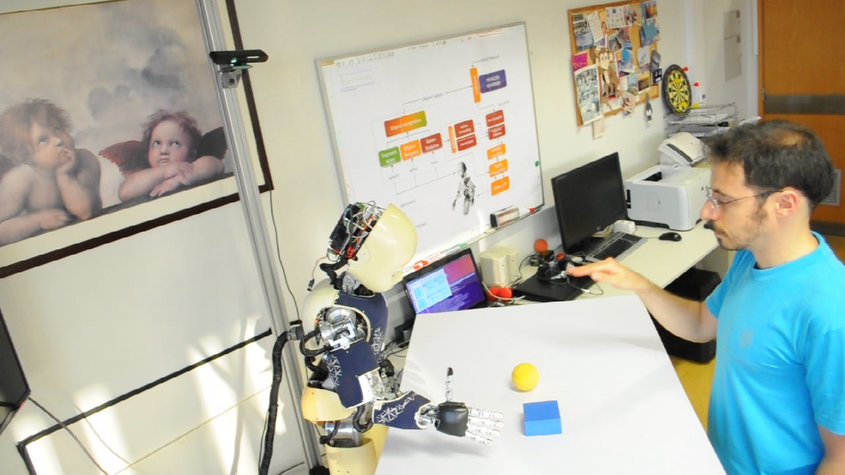
\includegraphics[width=\myWidthTwo\linewidth]{seq2-touch-7} } \quad
%     %
%     \subfloat
%     { 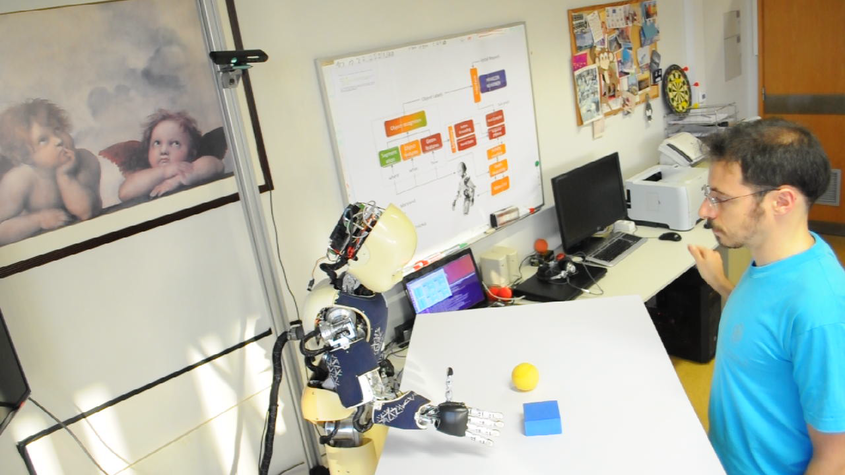
\includegraphics[width=\myWidthTwo\linewidth]{seq2-touch-8} } \quad
%     %
%     \subfloat
%     { 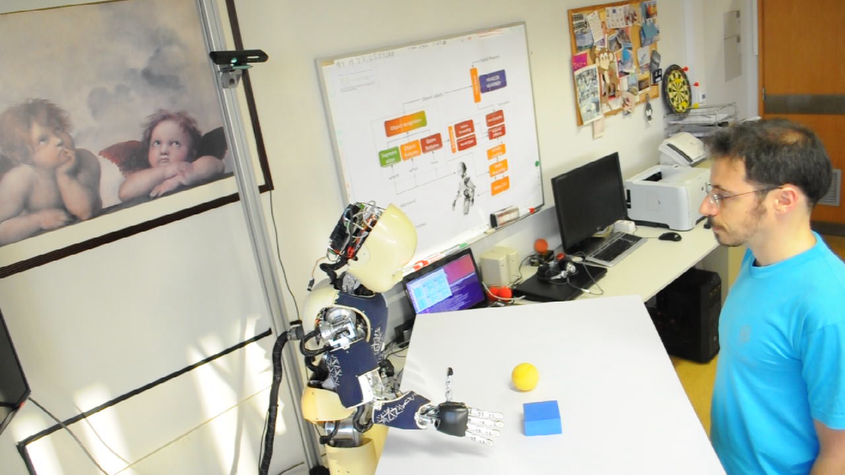
\includegraphics[width=\myWidthTwo\linewidth]{seq2-touch-9} }
%     \caption{touch}
% \end{figure*}

\IEEEPARstart{C}{ooperation} is a tenet of human society~\cite{turner:1975}, whereby humans have the ability of working successfully in groups.
In a team, understanding one another is a fundamental pre-requisite for success.
Team members typically agree on common goals~(e.g., through verbal and non-verbal communication), they work towards the execution of these goals in a coordinated way, and they understand each other's physical actions~(e.g., body movements) towards the realization of the final target.
Human team coordination and mutual understanding is effective~\cite{ramnani:2004:natureneuro} because of~(i) the capacity to \emph{adapt} to unforeseen events in the environment, and re-plan one's actions in real time if necessary, and~(ii) a common motor repertoire and action model, which permits us to understand a partner's physical actions and manifested intentions as if they were our own.
However, the performance of \hh{} teams is still superior to that of \hr{} teams.

Social robots\footnote{A social robots is ``[a robot that is] able to communicate and interact with us, understand and even relate to us, in a personal way. [It] should be able to understand us and itself in social terms''~\cite{breazeal:2002:dsr}.} are becoming ever more present in domestic, public and leisure environments, thanks to the rapid technical advancements that touch all aspects of robotics: sensors, actuators, and algorithms.
However, putting socially intelligent machines alongside common human users~(as opposed to specialized factory technicians as has been done in industrial robotics since the 1960s), bears issues and challenges.
In particular, the communication skills possessed by a robot cannot be entirely pre-programmed, because we cannot possibly model all the possible verbal and non-verbal~(e.g., gestures) cues that can take place during \hri, due to the richness of language and the high variability of the real world outside of laboratories of factories.
For this reason it is necessary to have robots that \emph{learn} elements of language, and learn how to link these elements with other skills, such as other perceptual modalities~(e.g., vision of objects of the world, vision of other agents' physical actions) and manipulation abilities~(e.g., grasping objects and moving them to achieve a goal).
This is often achieved with probabilistic and statistical methods. TODO ADD REF

The growing field of developmental robotics~\cite{lungarella:2003:devrobsurvey,cangelosi:2015:devrobbook} takes inspiration from the progressive learning phenomena observed in children's mental development~(e.g., the understanding of language, the acquisition of manipulation skills, the understanding of others' actions), and investigates how to model the evolution and the learning of these increasingly complex cognitive processes.
In this line of research, robots are experimental platforms, being used to verify theoretical models of emergence and development of cognition.
The rationale is the following: if a model is instantiated inside a system physically embedded in the real world, many things can be learned about its strengths and limitations.

In neuroscience research, visuomotor neurons~(i.e., neurons that are activated by visual stimuli) have been a subject of ample study~\cite{rizzolatti:2001:nrn}.
Mirror neurons are one class of such neurons that responds to action and object interaction, both when the agent acts and when it observes the same action performed by others, hence the name ``mirror''.
We show that, using this theory, a robot can first acquire knowledge by sensing and self-exploring its surrounding environment~(e.g., by interacting with available objects and building up an affordance representation of the interactions and their outcomes) and, as a result, the robot is capable of generalizing its acquired knowledge while observing another agent~(e.g., a human person) who performs similar physical actions to the ones executed during prior robot training.
This tackles the so-called correspondence problem~\cite{nehaniv:2002:correspondence} in our simple collaboration sceanario, assuming that the two agents have a similar body~(i.e., a humanoid robot and a human) and operate on a shared space~(i.e., a table accessible by both agents' arms).

This article is an extention of our previous work~\cite{saponaro:2017:glu}.
We combine robot ego-centric learning about language and object affordances~\cite{salvi:2012:smcb} with the observation of external agents by gesture recognition~\cite{saponaro:2013:crhri}.
We formalize a probabilistic method to fuse the self-learned knowledge with the observation of others, and we report experimental findings about the generalization power of our system, particularly on how our model is able to generate non-obvious verbal descriptions of \hri{} scenarios in the context of manipulation.

%BELOW IS THE GLU TEXT

%Robotics is progressing fast, with a steady and systematic shift from the industrial domain to domestic, public and leisure environments~\cite[ch.~65, Domestic Robotics]{siciliano:2016:handbook2}. Application areas that are particularly relevant and being researched by the scientific community include: robots for people's health and active aging, mobility, advanced manufacturing~(Industry~4.0). In short, all domains that require direct and effective \hri{} and communication (including language and gestures~\cite{matuszek:2014:aaai}).

%However, robots have not reached the level of performance that would enable them to work with humans in routine activities in a flexible and adaptive way, for example in the presence of sensor noise, or unexpected events not previously seen during the training or learning phase. One of the reasons to explain this performance gap between \hh{} teamwork and a \hr{} teamwork is in the collaboration aspect, i.e., whether the members of a team understand one another. Humans have the ability of working successfully in groups. They can agree on common goals~(e.g., through verbal and non-verbal communication), work towards the execution of these goals in a coordinated way, and understand each other's physical actions~(e.g., body gestures) towards the realization of the final target. Human team coordination and mutual understanding is effective~\cite{ramnani:2004:natureneuro} because of~(i) the capacity to \emph{adapt} to unforeseen events in the environment, and re-plan one's actions in real time if necessary, and~(ii) a common motor repertoire and action model, which permits us to understand a partner's physical actions and manifested intentions as if they were our own~\cite{saponaro:2013:crhri}.

%In neuroscience research, visuomotor neurons~(i.e., neurons that are activated by visual stimuli) have been a subject of ample study~\cite{rizzolatti:2001:nrn}. Mirror neurons are one class of such neurons that responds to action and object interaction, both when the agent acts and when it observes the same action performed by others, hence the name ``mirror''.

% \begin{figure}
%   \centering
%   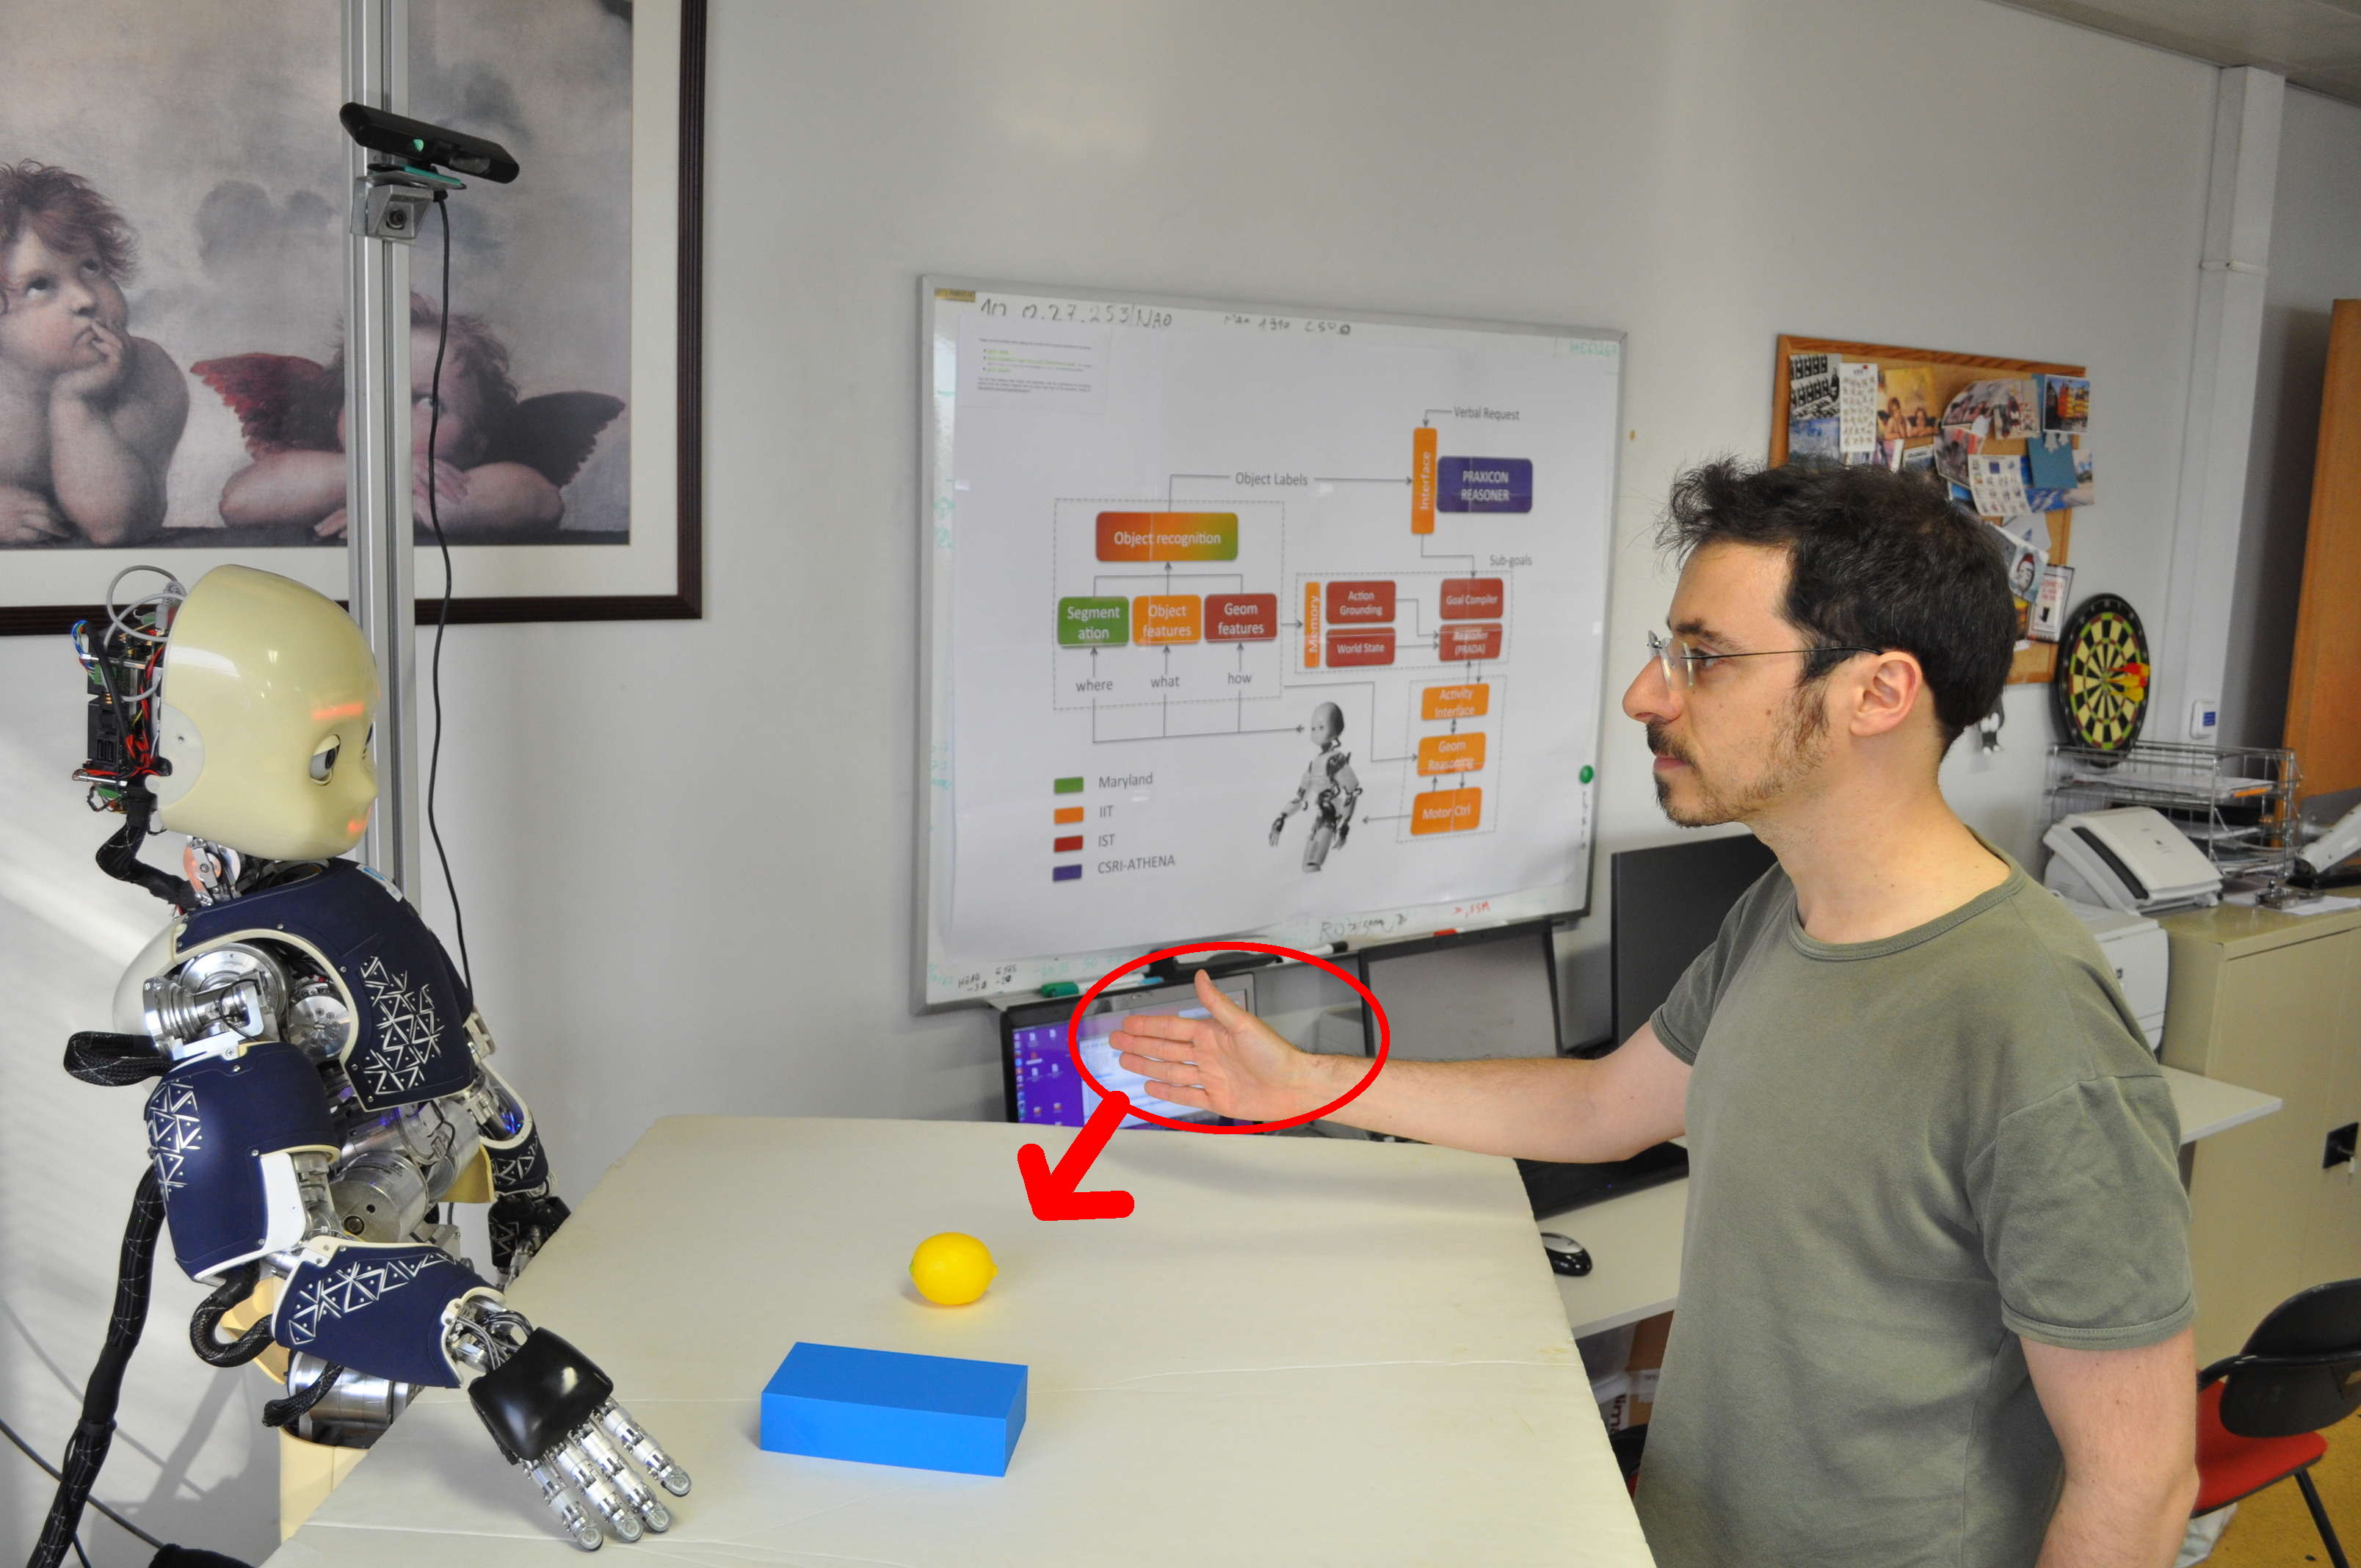
\includegraphics[width=0.9\columnwidth]{human_tap}
%   \caption{Experimental setup, consisting of an iCub humanoid robot and a human user performing a manipulation gesture on a shared table with different objects on top. The depth sensor in the top-left corner is used to extract human hand coordinates for gesture recognition. Depending on the gesture and on the target object, the resulting effect will differ.}
%   \label{fig:experimental_setup}
% \end{figure}

% This work takes inspiration from the theory of mirror neurons, and contributes towards using it on humanoid and cognitive robots. We show that a robot can first acquire knowledge by sensing and self-exploring its surrounding environment~(e.g., by interacting with available objects and building up an affordance representation of the interactions and their outcomes) and, as a result, the robot is capable of generalizing its acquired knowledge while observing another agent~(e.g., a human person) who performs similar physical actions to the ones executed during prior robot training. Fig.~\ref{fig:experimental_setup} shows the experimental setup.
